\documentclass[12 pt,a4paper,twocolumn]{article}
\usepackage[utf8]{inputenc}
\usepackage[T1]{fontenc}
\usepackage[italian,english]{babel}
\usepackage{indentfirst} 
\usepackage{graphicx}
\usepackage{tabularx}
\usepackage{siunitx}
\usepackage{amsmath,stix,bm}
\usepackage{eucal}
\usepackage{caption}

\usepackage{multicol}
\usepackage[includeheadfoot,margin=0.7in,top=0.3 in,bottom=0.35in]{geometry}
%Per grafica vettoriale tramite InkScape%
\usepackage{color}
\usepackage{transparent}
\graphicspath{{img/}}
\usepackage[dvipsnames]{xcolor}
\usepackage{pdfpages}
\usepackage{pgfplots}
\usepackage{textcomp}

\usepackage{xcolor,colortbl}
\usepackage{listings}
\usepackage{cleveref}
\usepackage{caption}
\DeclareCaptionFont{quack}{}
\captionsetup[figure]{font={color=gray,small},labelfont={color=black,sc}}
\captionsetup[table]{font={color=gray,small},labelfont={color=black,sc}}
\captionsetup[subfigure]{font={color=gray,small},labelfont={color=black}}
\addto\captionsenglish{\renewcommand{\figurename}{Fig.}}
\addto\captionsenglish{\renewcommand{\tablename}{Tab.}}
\addto\captionsitalian{\renewcommand{\tablename}{Tab.}}
\crefname{table}{Tab.}{Tabs.}  

\usepackage{cancel}

\usepackage{subcaption}
\usepackage{titlesec}
\titleformat*{\section}{\Large\bfseries\color{myGeneralColor}}
\titleformat*{\subsection}{\large\bfseries\color{myGeneralColor}}
\titleformat*{\subsubsection}{\itshape\bfseries\color{myGeneralColor}}
\definecolor{burntsienna}{rgb}{0.91, 0.45, 0.32}
\definecolor{carrotorange}{rgb}{0.93, 0.57, 0.13}
\definecolor{darktangerine}{rgb}{1.0, 0.66, 0.07}
\definecolor{deepsaffron}{rgb}{1.0, 0.6, 0.2}
\definecolor{flax}{rgb}{0.93, 0.86, 0.51}
\definecolor{lava}{rgb}{0.81, 0.06, 0.13}
\usepackage{pifont}% http://ctan.org/pkg/pifont
\newcommand{\cmark}{\ding{51}}%
\newcommand{\xmark}{\ding{55}}%
\definecolor{mintbg}{rgb}{.63,.79,.95}
\graphicspath{{figures/}{code/figs/}{../code/figs2/}{../code/figs/}} %Setting the graphicspath
\makeatletter
\def\input@path{{figures/}{code/figs/}{../code/figs/}{../code/figs/}}
\makeatother
\usepackage{import}
\usepackage{authblk}
\pgfplotsset{compat=newest}
\pgfplotsset{plot coordinates/math parser=false}
\newlength\figureheight
\newlength\figurewidth
\usepackage{placeins}
\usepackage{float}
\usepackage{blindtext}
\usepackage{authblk}
\renewcommand\Affilfont{\tiny \color{gray}}

\title{\vspace*{10 pt}\color{myGeneralColor}\Huge\textbf{Microreometro e proprietà viscoelastiche delle cellule}\vspace*{1 pt}}
\author[]{Mastrofini Alessandro}
\affil[]{\small alessandro.mastrofini@alumni.uniroma2.eu}
\renewcommand*{\Authand}{ e }
\date{}
\usepackage{fancyhdr}
\pagestyle{fancy}
\fancyhf{}
	\lhead{\small\color{gray} University of Rome Tor Vergata - MSSF}
\fancyfoot[C]{\small{\thepage\  di \pageref{LastPage}}}
\renewcommand{\headrulewidth}{0pt}

\fancypagestyle{plain}{
	\renewcommand{\headrulewidth}{0pt}
	%\setlength{\headheight}{80 pt} 
	\lhead{\small\color{gray} Modellazione e Simulazione di Sistemi Fisiologici  \\
	Docente: Caselli, Federica \\
	Università degli Studi di Roma Tor Vergata\\
	Ingegneria Medica - 2022}
	\rhead{
\includegraphics[height=45pt]{logo.png} }
	\fancyfoot{}
}
\usepackage{lastpage}
\addtocontents{toc}{\protect\setcounter{tocdepth}{0}}
\usepackage{lipsum}
\usepackage[
backend=bibtex,
style=numeric,
sorting=none
]{biblatex} %Imports biblatex package
\addbibresource{mybib.bib} %Import the bibliography file

\usepackage{listings}
\definecolor{codegreen}{rgb}{0,0.6,0}
\definecolor{codegray}{rgb}{0.5,0.5,0.5}
\definecolor{codestring}{rgb}{0.623, 0.176, 0.588}
\definecolor{backcolour}{rgb}{0.96,0.96,0.96}
\definecolor{bbcolour}{rgb}{0.01,0.03,0.35}
\definecolor{indexcolour}{rgb}{0,0.4,0.4}
\definecolor{myOrange}{rgb}{0.933, 0.313, 0.066}
\definecolor{myBlue}{rgb}{0, 0.298, 0.8}
\lstdefinestyle{mystyle}{
	backgroundcolor=\color{backcolour},   
	commentstyle=\color{codegreen},
	classoffset=1,
	keywordstyle=\color{bbcolour},
	numberstyle=\tiny\color{codegray},
	stringstyle=\color{codestring},
	basicstyle=\ttfamily\scriptsize,
	breakatwhitespace=false,  
	breaklines=true,                 
	captionpos=b,                    
	keepspaces=false,                 
	numbers=left,                    
	numbersep=3pt,                  
	showspaces=false,                
	showstringspaces=false,
	showtabs=false,                  
	tabsize=2
}
\lstset{texcl=false, mathescape=true,style=mystyle}
\lstset{emph={%  
		i, j,X%
	},emphstyle={\color{bbcolour}}%
}%
\definecolor{myGeneralColor}{rgb}{0, 0.227, 0.580}
\usepackage{tikz}
\usetikzlibrary{fit}
\usetikzlibrary{shapes.geometric, arrows}
\tikzstyle{startstop} = [rectangle, rounded corners, minimum width=7cm, minimum height=1cm,text centered,  fill=backcolour,text width=6.5 cm,draw=gray]
\tikzstyle{startstop2} = [rectangle, rounded corners, minimum width=5cm, minimum height=2cm,text centered,  fill=backcolour,draw=gray]
\tikzstyle{io} = [trapezium, trapezium left angle=80, trapezium right angle=100, minimum width=7cm, minimum height=1cm, text centered,text width=6.5 cm,  fill=backcolour,draw=gray]
\tikzstyle{io2} = [trapezium, trapezium left angle=70, trapezium right angle=110, minimum width=2cm, minimum height=1cm, text centered,  fill=backcolour,draw=gray]
\tikzstyle{process} = [rectangle, minimum width=7cm, minimum height=1cm, text centered,text width=6.5cm,  fill=backcolour,text badly centered,draw=gray]
\tikzstyle{decision} = [diamond, minimum width=1cm, minimum height=1cm, text centered,  fill=backcolour,draw=gray,text width=2cm]
\tikzstyle{arrow} = [thick,->,>=stealth]
\tikzstyle{process2} = [rectangle, minimum width=3.5cm, text width=3.2cm,minimum height=1cm, text centered, dashed, fill=backcolour,draw=gray]
\tikzstyle{process3} = [rectangle, minimum width=4cm,text width=4cm, minimum height=1cm, text centered,  fill=backcolour,draw=gray]
\tikzstyle{process4} = [rectangle, minimum width=6cm,text width=5.5cm, minimum height=1cm, text centered,  fill=backcolour,draw=gray]

\renewcommand*{\bibfont}{\normalfont\footnotesize}

\begin{document}


\twocolumn[{
\begin{@twocolumnfalse} 
		\vspace*{20 pt}
	\begingroup
	\let\center\flushleft
	\maketitle
	\let\endcenter\endflushleft
	\endgroup
	\begin{abstract}
% \noindent
% \noindent\\
% \noindent
% \noindent
% \noindent
La caratterizzazione delle proprietà meccaniche della cellula è di grande importanza per caratterizzarne lo stato biologico.

Tra le diverse tecniche il microreometro permette di caratterizzarne le proprietà viscoelastiche. Si considera un esperimento di misura di un microreometro a biglia paramagnetica e il dati sperimentali per analizzare il comportamento di un modello meccanico di cellula a parametri concentrati.

Tale modello viene descritto dal parallelo di un corpo di Maxwell con una rigidezza elastica al quale viene aggiunto uno smorzatore in serie per  ridurre la discrepanza con i dati sperimentali.

Le costanti viscoelastiche stimate dal modello a parametri concentrati sono indicative delle proprietà dell'intera cellula e non dei singoli costituenti quali membrana, citoscheletro o citoplasma, per i quali sarebbe richiesto un modello differente.
%% ABSTRACT 

	\end{abstract}
	\vspace*{20 pt}
\end{@twocolumnfalse}
}]

\section{Introduzione}



\textcolor{blue}{\lipsum[1]}

\section{Background}

\textcolor{blue}{\lipsum[1-4]}

\begin{figure}[t!]
	\centering
	\footnotesize{
	 \def\svgwidth{\linewidth}
	 \input{rheometer.pdf_tex}}
	\caption{}
	\label{fig:system}
\end{figure}


\begin{figure*}[h!]
	\begin{subfigure}{0.5\linewidth}
	\centering
	\footnotesize{
	\def\svgwidth{0.9\linewidth}
	\input{mechanic_model.pdf_tex}}
\caption{}
\label{fig:mechanical}
	\end{subfigure}\hfill
	\begin{subfigure}{0.5\linewidth}
	\centering
	\footnotesize{
	\def\svgwidth{0.9\linewidth}
	\input{creep_response.pdf_tex}}
\caption{}
\label{fig:mechanical1}
\end{subfigure}\hfill
\caption{text}
\end{figure*}



\subsection{Microreometro a biglia magnetica}




\section{Risultati}

\begin{figure*}[t!]
\begin{lstlisting}[language=matlab]
	function dydt=zener_displacement(t,y,parameters,tspan,flag)
		k_0=parameters(1);
		k_1=parameters(2);
		gamma_0=parameters(3);
		gamma_1=parameters(4);
		F_bar=parameters(5);
		switch flag
			case 'square'
				[F, dF]=force(t,tspan);
				dydt=((F-k_0*y)/gamma_1 + (dF/k_1))*(1+k_0/k_1);
			case 'step'
				dydt=(-(k_0/gamma_1)*y+(F_bar/gamma_1))/(1+(k_0/k_1));
			case 'harmonic'
				omega=parameters(7);
				F=F_bar*(1+sin(omega*t));
				dF=F_bar*omega*cos(omega*t);
				dydt=((F-k_0*y)/gamma_1 + (dF/k_1))*(1+k_0/k_1);
		end
	end
\end{lstlisting}
\caption{Routine richiamata da \texttt{ode15s} per la soluzione dell'equazione differenziale per lo spostamento del corpo Zener}
\vspace{0.8cm}
\begin{lstlisting}[language=matlab]
	function dydt=dashpot_displacement(t,y,parameters,tspan,flag)
		gamma_0=parameters(3);
		gamma_1=parameters(4);
		F_bar=parameters(5);
		switch flag
			case 'square'
				[F, dF]=force(t,tspan);
				dydt=F/gamma_0;
			case 'step'
				dydt=F_bar/gamma_0;
			case 'harmonic'
				omega=parameters(7);
				F=F_bar*(1+sin(omega.*t));
				dF=F_bar*omega*cos(omega*t);
				dydt=F/gamma_0;
		end
	end	
\end{lstlisting}
\caption{Routine richiamata da \texttt{ode15s} per la soluzione dell'equazione differenziale per lo spostamento dello smorzatore}
\end{figure*}


\begin{figure*}[t!]
	\begin{lstlisting}[language=matlab]
function [F, dF]=force(t_curr,t)	
	T_cyc=5;
	N_cyc=4;
	F=2000;
	freq=1/T_cyc;
	squareWave=F/2*(square(2*pi*freq*t,50)+1);
	squareWave(end)=0;
	squareWave_smooth=smoothdata(squareWave,'gaussian',(size(t)/N_cyc)*0.05);
	derivate=[0 diff(squareWave_smooth)];
	F=interp1(t,squareWave_smooth,t_curr);
	dF=interp1(t,derivate,t_curr);
end
	\end{lstlisting}
	\caption{Routine per la generazione dell'onda quadra regolarizzata di ingresso. Viene inserita anche la funzione \texttt{interp1} per permette a \texttt{ode15s} di leggere il valore di forza a qualsiasi instante temporale ($\mathtt{t\_curr}$) e non solo sui campione dove è stato definito il segnale.}
\end{figure*}

\begin{figure}[t!]
	\centering
	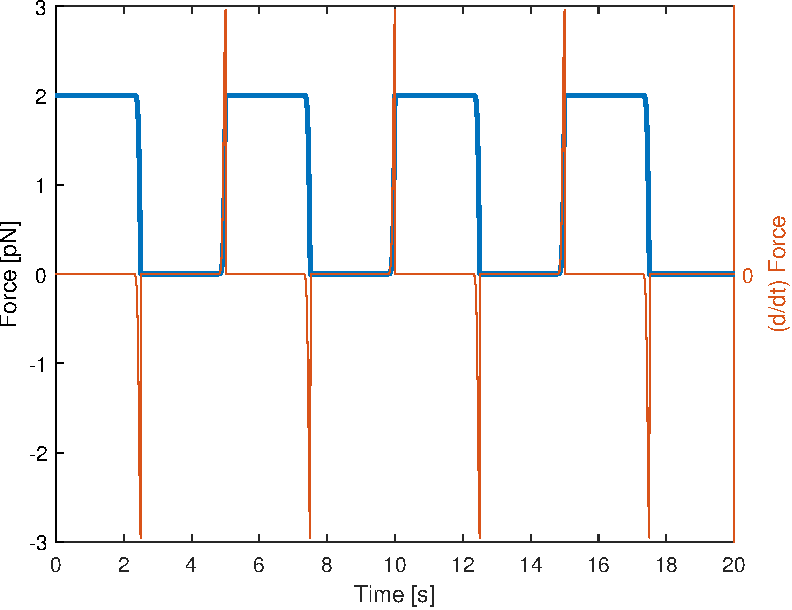
\includegraphics[width=0.95\linewidth]{../code/figs/square_regularized}
	\caption{}
	\label{fig:squareregularized}
\end{figure}



\begin{figure*}[t!]
	\begin{subfigure}{0.5\linewidth}
	\centering
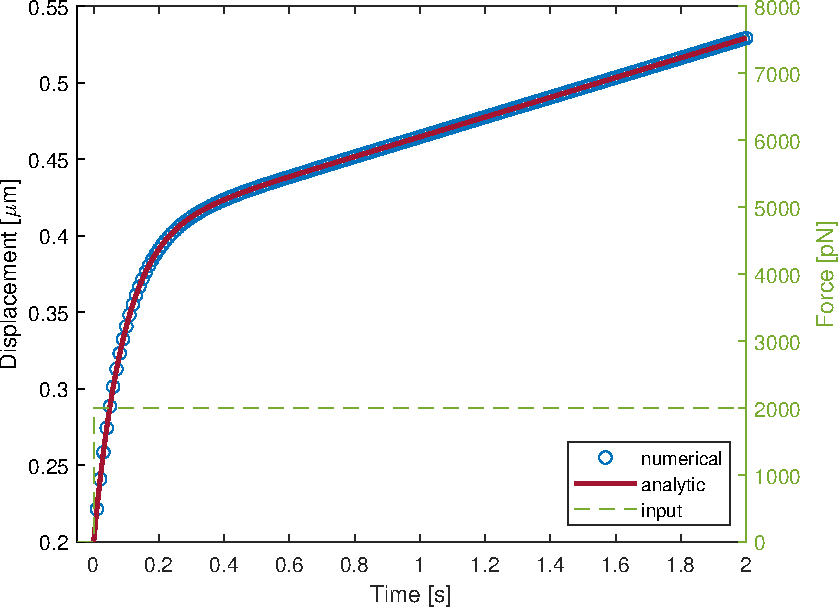
\includegraphics[width=0.95\linewidth]{../code/figs/step}
\caption{}
\label{fig:square}
	\end{subfigure}\hfill
	\begin{subfigure}{0.5\linewidth}
	\centering
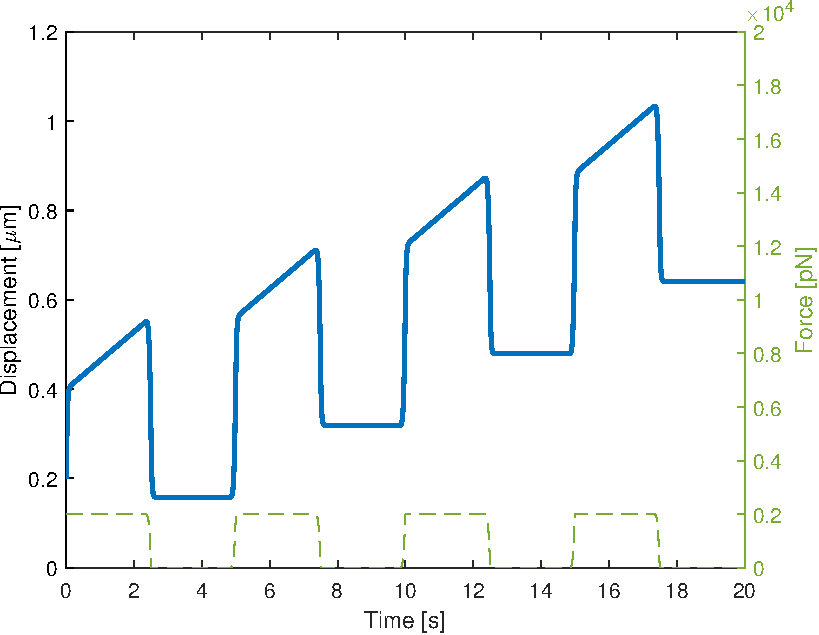
\includegraphics[width=0.95\linewidth]{../code/figs/square}
\caption{}
\label{fig:step}
\end{subfigure}\hfill
\caption{Risposta del sistema ad ingresso a gradino (a) e ad onda quadra con periodo di 5s (b).}
\end{figure*}

\begin{figure*}[t!]
	\centering
	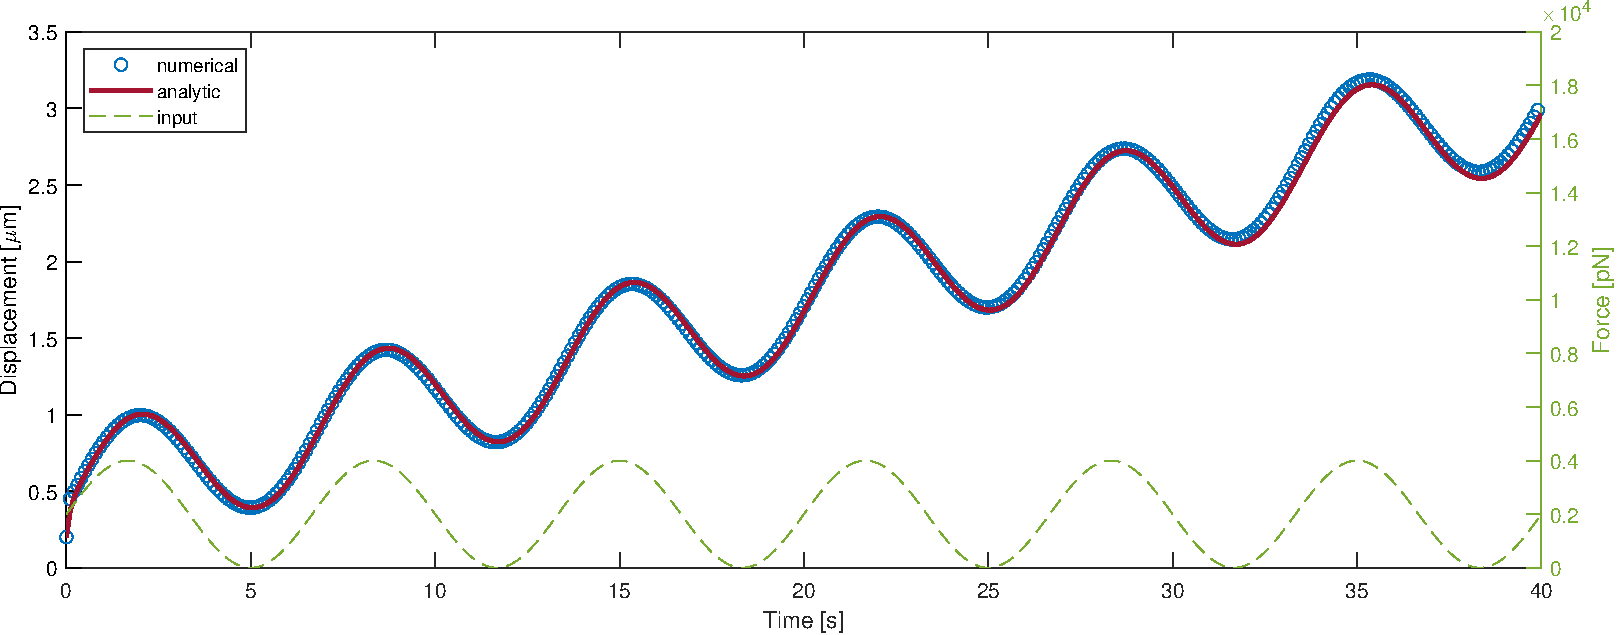
\includegraphics[width=0.95\linewidth]{../code/figs/harmoniclarge}
	\caption{Confronto tra il risultato analitico e il risultato numerico con ingresso sinusoidale a frequenza 0.15 Hz applicato per 40s.}
	\label{fig:harmoniclarge}
\end{figure*}

\begin{figure*}[t!]
	\begin{subfigure}{0.33\linewidth}
		\centering
			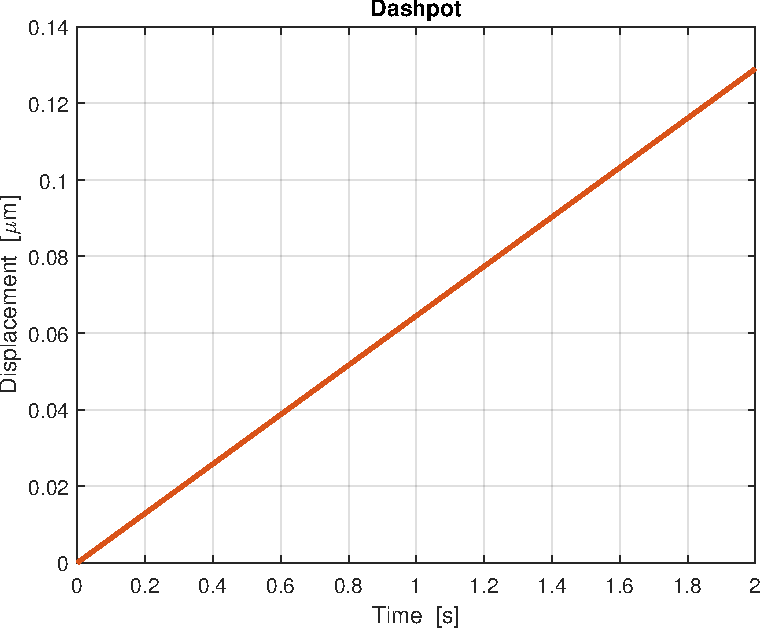
\includegraphics[width=0.95\linewidth]{../code/figs/step_dashpot_}
		\caption{}
	\end{subfigure}\hfill
	\begin{subfigure}{0.33\linewidth}
	\centering
		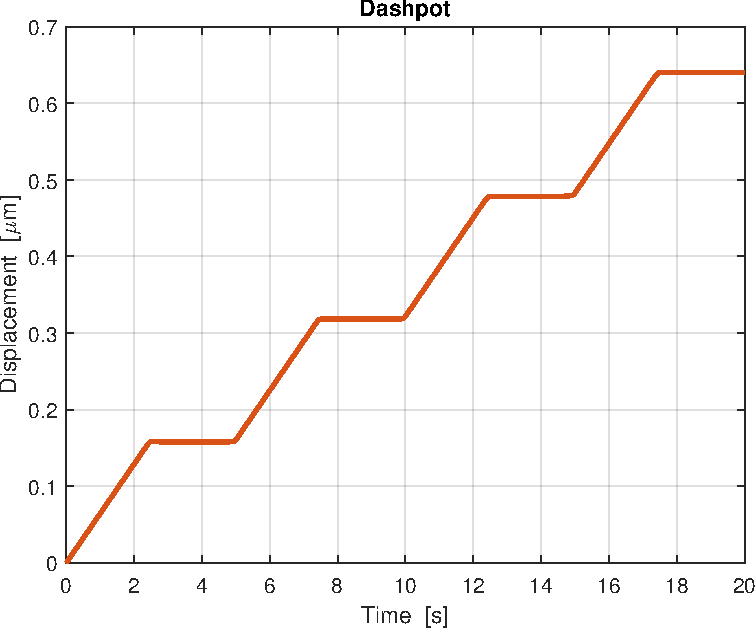
\includegraphics[width=0.95\linewidth]{../code/figs/square_dashpot_}
	\caption{}
\end{subfigure}\hfill
	\begin{subfigure}{0.33\linewidth}
	\centering
	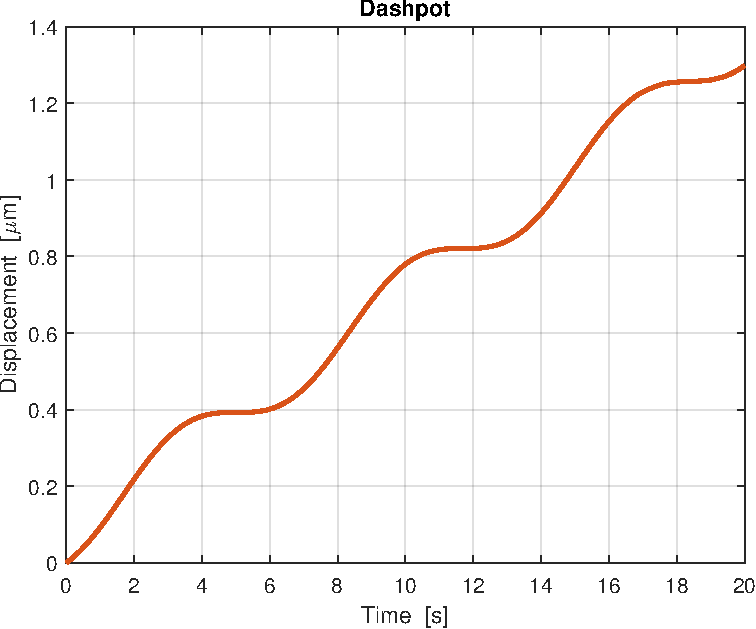
\includegraphics[width=0.95\linewidth]{../code/figs/harmonic_dashpot_}
	\caption{}
\end{subfigure}\hfill
	\begin{subfigure}{0.33\linewidth}
		\centering
			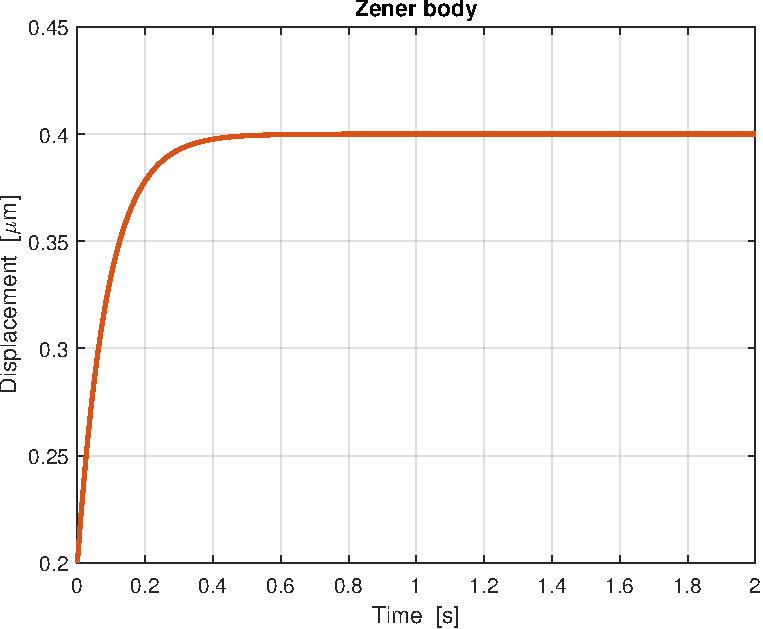
\includegraphics[width=0.95\linewidth]{../code/figs/step_zener_}
		\caption{}
	\end{subfigure}\hfill
	\begin{subfigure}{0.33\linewidth}
		\centering
		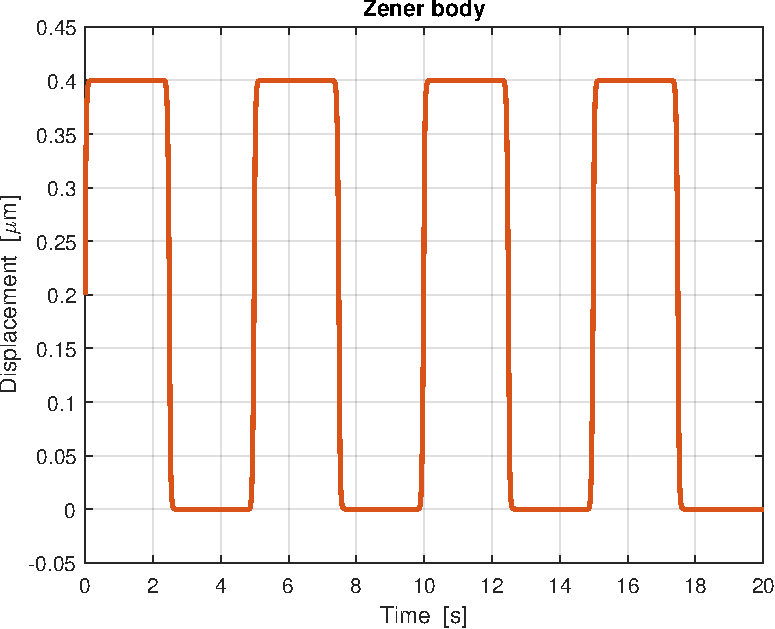
\includegraphics[width=0.95\linewidth]{../code/figs/square_zener_}
		\caption{}
	\end{subfigure}\hfill
	\begin{subfigure}{0.33\linewidth}
		\centering
		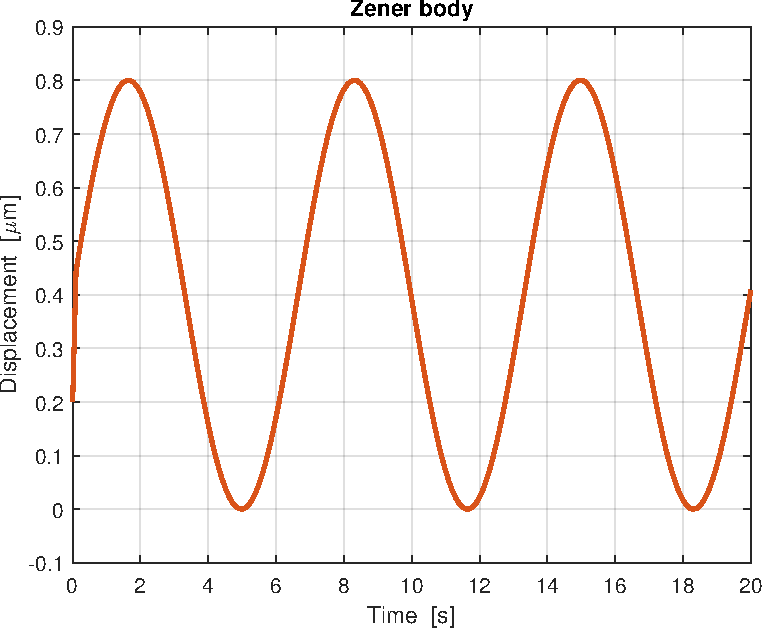
\includegraphics[width=0.95\linewidth]{../code/figs/harmonic_zener_}
		\caption{}
	\end{subfigure}\hfill
	\caption{Andamento dello spostamento dello smorzatore (sopra) e del corpo Zener (sotto) nel caso di ingresso a gradino (a,d); a onda quadra con periodo di 5s (b,e); sinusoide a frequenza 0.15 Hz (c,f).}
\end{figure*}

\subsection{Ingresso a gradino}




\textcolor{blue}{\lipsum[1-2]}

\subsection{Ingresso a onda quadra}




\textcolor{blue}{\lipsum[1-2]}

\subsection{Ingresso sinusoidale}




\textcolor{blue}{\lipsum[1-2]}



\section{Conclusioni}

\textcolor{blue}{\lipsum[1-2]}


\raggedbottom


\raggedbottom
\pagebreak
\section*{Disponiblità dei dati}

Il materiale è disponibile alla repository online del progetto: \url{https://github.com/mastroalex/ecm-mmt}.

\printbibliography[title=Riferimenti]
%\section*{References}

\clearpage
\onecolumn
\section*{Appendice}



\end{document}